\documentclass[11pt]{article}
\usepackage[margin=1.1in]{geometry}
\usepackage{amsmath,amssymb}
\usepackage{booktabs}
\usepackage{graphicx}
\usepackage[hidelinks]{hyperref}
\usepackage{xcolor}
\usepackage{pgfplots}
\pgfplotsset{compat=1.17}
\definecolor{accent}{RGB}{42,101,175}
\definecolor{corrupt}{RGB}{201,109,44}
\definecolor{inkmut}{RGB}{110,118,126}

\title{Instructions Buy the Phrase; the Phrase Costs Preference:\\
An Epistemic Audit of LLM Aggregation Pipelines at Auditable Scale}
\author{Sam Bobo}
\date{Draft v0.3, September 2026}

\newcommand{\ci}[2]{\ensuremath{[#1,\,#2]}}

\begin{document}
\maketitle

\begin{abstract}
Mixture-of-Agents (MoA) pipelines, in which an aggregator model
synthesizes the outputs of several proposer models, achieve
state-of-the-art results on preference-judged benchmarks. Every
published gain, however, is measured by an LLM preference judge, and
the literature does not establish what such gains consist of. This
paper audits the MoA architecture at auditable scale (7 to 20B local
models) with pre-registered experiments, validated instruments, and
causal designs, and reports three linked findings. (1)~A phrase-swap
experiment shows that an epistemic instruction (``label estimates with
phrase $X$'') produces only its named phrase: the dictated form appears
in two thirds of outputs regardless of which synonym is named, while
the construct rate outside the named phrase is statistically unchanged
(CIs $\ci{-0.079}{+0.111}$, $\ci{-0.103}{+0.087}$). (2)~Order-debiased
preference judging shows a real aggregation lift: the aggregated
pipeline beats the same writer answering directly in $0.818$
\ci{0.718}{0.919} of decisive pairs, surviving length matching and
replicating under a second judge from a disjoint model family ($0.788$
\ci{0.645}{0.917}). The same judges penalize the instructed arms: the
phrase-bearing arms lose to their own control ($0.261$
\ci{0.140}{0.388}; $0.317$ \ci{0.152}{0.480}), and the penalty holds
in three of four judge-by-form cells, with the fourth agreeing in point
estimate at lower power. Because the arms differ only in the phrase,
the penalty is causally attributable to it. Together these results
identify a measured tension: instruction tuning of epistemic
disposition installs surface forms, and preference optimization
removes exactly those forms. (3)~The preference instrument itself is
majority reading-order at this scale, as a property of the task
format: raw first-position preference is $0.85$ to $0.88$ across four
judges from four model families, and order-debiasing converts $60$ to
$95\%$ of pairs to ties. Mechanism results further bound the MoA
narrative: the aggregator selects sources rather than recomputing,
ignores cross-proposer corroboration, and transports only a small
fraction of the epistemic qualification it is given, with
within-corpus slopes of $0.11$ to $0.33$ replicated across two writers
and two corpora. The audit's design consequences were then engineered
and prospectively re-tested as their own registered experiments.
Assigning a contested quantity to a second proposer halves
corrupted-value adoption (from $0.90$ to $0.45$); carrying epistemic
qualification out-of-band, in a mechanically assembled appendix the
writer never sees, preserves all of it against the $17\%$ that
survives prose, measurably changes downstream decisions ($+0.69$ over
a matched irrelevant-appendix control, at parity with in-prose
placement), and shows no detected preference cost; and the
re-consultation loop closes end-to-end with a live proposer (adoption
$0.905$ versus $0.333$, within noise of a scripted ceiling). The
measurement kit, the dictation registry, and all pre-registrations are
released.
\end{abstract}

\section{Introduction}
\label{sec:intro}

Mixture-of-Agents \cite{wang2024moa} reports that a stack of
open-source proposers plus an aggregator surpasses GPT-4o on
AlpacaEval~2.0 (65.1\% versus 57.5\% length-controlled win rate) and
frames the result as collaborativeness: models produce better responses
when shown other models' outputs, even lower-quality ones. Every number
in that paper, and in the surrounding multi-agent literature, is
produced by an LLM preference judge. No published MoA evaluation
measures a verifiable outcome, tests error propagation, validates its
judge on the deployed task, or separates behavioral change from surface
compliance.

This paper supplies that audit. It is the product of a
falsification-first research program that ran more than fifty
pre-registered experiments on a MoA-architecture pipeline small enough
to audit completely: 7 to 20B open models on consumer hardware, with
every registration, deviation, and verdict recorded in a public ledger
before and after each run. The architecture is a two-layer MoA with
three proposers and one aggregator. Earlier experiments in the program
ran the MoA aggregate-and-synthesize prompt verbatim; the causal
experiments of Sections~\ref{sec:phrase} and \ref{sec:pref}
deliberately use a minimal aggregator prompt instead, so that
instruction content is the manipulated variable rather than a
background condition.

Three questions organize the audit.

\begin{enumerate}
\item \textbf{What do epistemic instructions to an aggregator actually
do?} (Section~\ref{sec:phrase}) A counterbalanced phrase-swap
experiment shows that they install the named phrase and nothing
measurable beyond it.
\item \textbf{Does the MoA preference lift replicate at auditable
scale, and what is it made of?} (Section~\ref{sec:pref}) It
replicates, at $0.818$ of decisive pairs and surviving a length
control, and its composition is not explained by the full surface
feature set. The same judge penalizes instructed epistemic marking,
causally.
\item \textbf{Do the mechanisms the MoA narrative assumes exist?}
(Section~\ref{sec:mech}) Largely no. The aggregator prefers
uncorrupted sources but does not recompute; corroboration among
proposers does not increase transport; and two same-base domain
fine-tunes do not share a reasoning signature.
\end{enumerate}

The audit's instruments are themselves audited
(Section~\ref{sec:instruments}). Fourteen recorded instrument-validity
findings drive the methodology, including the discovery, made
mechanically by a dictation registry, that an earlier judge prompt in
the same program enumerated the phrases that the system prompts
dictated to writers, entangling instrument with scaffold at the
instrument layer.

\paragraph{Contributions.} The paper makes the following contributions.
\begin{enumerate}
\item The first causal separation of compliance from behavior in
epistemic instruction-following (the phrase-swap design), with a
two-link causal chain showing that preference optimization and
epistemic disposition are in tension.
\item A replication of the MoA preference lift at 20B scale under an
order-debiased protocol, with a decomposition showing that it is not
length, domain-framework density, or hedging register.
\item A measured characterization of local pairwise preference judging
as majority reading-order.
\item Mechanism results bounding the collaborativeness narrative, and
one positive result: orchestrator-routed re-consultation, closed
end-to-end with a live proposer, with evidence that both halves of the
loop are recognition-limited rather than capability-limited.
\item A prospectively re-tested architecture distilled from the audit
(engineered redundancy, out-of-band epistemic qualification,
evidence-bound seating) in which every component carries its own
registered verdict, including two informative nulls that demoted the
design's own rationales (Section~\ref{sec:harness}).
\item An open measurement kit (\texttt{gst}), a dictation registry
with a zero measured over-attribution rate, and the complete
pre-registration ledger.
\end{enumerate}

\section{Related Work}
\label{sec:related}

\paragraph{Aggregation pipelines.} MoA \cite{wang2024moa} is the
direct object of this audit. Li et al.\ \cite{li2025selfmoa} showed
that aggregating repeated samples of the single best model (Self-MoA)
outperforms mixed MoA by 6.6\% length-controlled win rate on AlpacaEval,
converging from the benchmark side with the finding reported here that
mixing is not automatically diverse (Section~\ref{sec:mech}). Ensemble
alternatives (rankers, routers, fusers) are surveyed in
\cite{wang2024moa}; the source-selector finding of this paper is the
LLM-ranker-adjacent result. Wang et al.\ \cite{wang2024rebuttal}
report that a single strongly prompted agent can match multi-agent
discussion, consistent with the council nulls reported here.

\paragraph{Judge pathologies.} Position bias and verbosity bias in LLM
judges are documented by Zheng et al.\ \cite{zheng2023judging}; length
correlations in preference optimization by Singhal et al.\
\cite{singhal2023length}; and sycophancy under preference pressure by
Sharma et al.\ \cite{sharma2023sycophancy}. The contribution here is
quantitative and causal at the pipeline level: an $85\%$ raw
first-position rate for a 20B judge, and a counterbalanced
demonstration that specific dictated epistemic phrases lose preference.

\paragraph{Instruction following.} The phrase-swap design is, to the
author's knowledge, the first to test an epistemic instruction by
swapping its named surface form under otherwise byte-identical prompts,
isolating form-independent behavioral residue from compliance.

\section{Experimental Setup}
\label{sec:setup}

\subsection{The pipeline}

The audited pipeline is a two-layer MoA. Three proposer seats
(prompted or domain-fine-tuned 7 to 8B models, or role-prompted samples
of the writer) produce contributions that are concatenated for a 20B
mixture-of-experts writer (\texttt{gpt-oss:20b}) under either the MoA
aggregate-and-synthesize prompt or a minimal lead-analyst prompt. The
case battery consists of eighteen strategic advisory scenarios spanning
healthcare, legal, and finance content.

\subsection{The registration ledger}

Every experiment is registered before it runs. A registration states
the hypotheses, the falsification conditions, the attainability
computations (the fraction of runs in which the outcome variable can
fire, computed from existing data, for every registered prediction),
and the consequences. Verdicts are entered in a status ledger that
distinguishes live, provisional, withdrawn, and blocked claims. Three
program-level audits re-classified earlier results, and null results
are cited only at the strength their audit class permits (informative,
weak, uninformative, or degenerate). All values reported below are live
ledger entries unless marked otherwise. The ledger's unit of
registration is termed a cell; the term is used here where a specific
ledger entry is cited. Confidence intervals are cluster-bootstrap
intervals over cases unless stated otherwise.

\section{Instrument Validation}
\label{sec:instruments}

Fourteen recorded instrument-validity findings shape the methodology.
Four are most relevant here.

\paragraph{Entanglement (finding 8).} If a prompt dictates the strings
an instrument detects, the measurement $M$ confounds compliance $C$
with behavior $B$: $M = C + B$, and a perfect detector still counts an
echoed phrase, because the difference between $C$ and $B$ is causal
rather than textual. A pattern-level decomposition (PD-13) first
exposed this: an instruction moved its dictated phrasings from $0/30$
to $28/30$ while non-dictated phrasings of the same construct moved
from $1/30$ to $4/30$ (difference-in-differences $+0.83$
\ci{+0.67}{+1.00}).

\paragraph{The dictation registry.} Every construct-bearing phrase that
any system, generation, or judge prompt places in a model's mouth was
extracted (125 entries from 35 prompt symbols; AST parsing and quote
scanning, no semantic classifier), frozen under a hash, and used to
gate all subsequent prompts. On its first run the registry found that
an earlier pairwise judge prompt in the same program enumerated the
seven phrases that the training-pair generators dictated to writers:
instrument entanglement at the instrument layer (finding 12). Measured
over-attribution is zero. Across 2{,}907 clean-provenance spans
(438{,}797 characters) and 60 de-scaffolded runs, no registry phrase
appears without dictation upstream, and direct probes confirm $0/60$
for every signature phrase (finding 13). Registry surface is therefore
diagnostic of the scaffold, which is what licenses literal-match
partitioning even where a judged paraphrase stage is withdrawn.

\paragraph{The validated judge.} Construct presence is scored by a
two-judge, batched, sentence-level protocol whose definitions name no
phrase and instruct judges not to reward particular wording. The
protocol passes the registry gate, and agreement on the deployed corpus
is $0.910$ (14{,}088/15{,}485 decisions). Document-level judging of the
same corpus scored $0.622$ and was rejected (finding 9).

\paragraph{Preference judging is majority reading-order (finding 14).}
Across the preference experiments (Section~\ref{sec:pref}), four
judges from four model families (a 20B MoE, a 30B MoE, a 14B dense
model, and a 7B dense model) showed raw first-position preference of
$0.85$ to $0.88$ wherever they parsed at all. Judging every pair in
both orders and requiring agreement converted $60$ to $95\%$ of pairs
to ties, with only the escape rate varying by judge (decisive rates
$0.05$ to $0.40$). The bias magnitude is invariant across vendor,
architecture, and generation: it is a property of the pairwise task
format rather than of a model. Order-debiased protocols keep preference
verdicts honest at the cost of most of the sample.

\section{Compliance Versus Behavior: The Phrase-Swap Experiment}
\label{sec:phrase}

\begin{figure}[t]
\centering
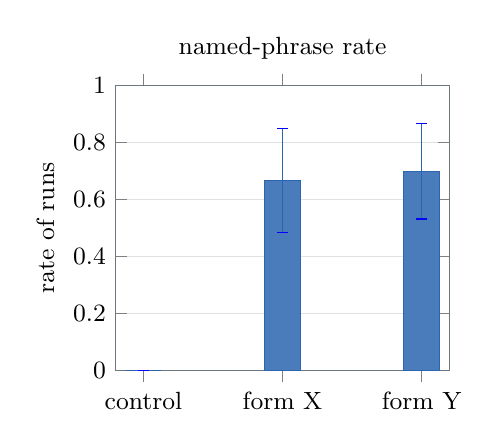
\begin{tikzpicture}
\begin{axis}[width=0.48\textwidth,height=5.2cm,ybar,bar width=13pt,
  ymin=0,ymax=1.0,ylabel={rate of runs},title={\small named-phrase rate},
  symbolic x coords={control,form X,form Y},xtick=data,
  axis line style={inkmut},tick label style={font=\small},
  ylabel style={font=\small},ymajorgrids,grid style={inkmut!22},
  error bars/y dir=both,error bars/y explicit]
\addplot+[fill=accent!85,draw=accent] coordinates {
  (control,0.000) +- (0,0)
  (form X,0.667) +- (0.207,0.182)
  (form Y,0.698) +- (0.174,0.167)};
\end{axis}
\end{tikzpicture}\hfill
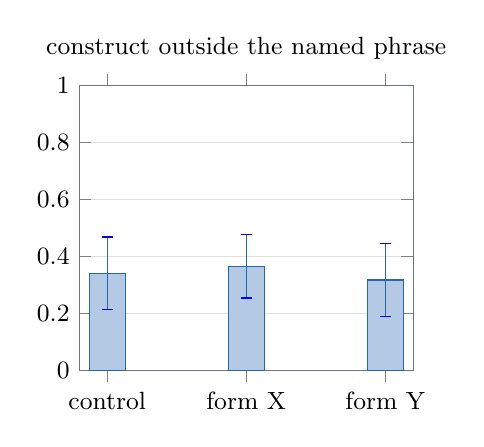
\begin{tikzpicture}
\begin{axis}[width=0.48\textwidth,height=5.2cm,ybar,bar width=13pt,
  ymin=0,ymax=1.0,title={\small construct outside the named phrase},
  symbolic x coords={control,form X,form Y},xtick=data,
  axis line style={inkmut},tick label style={font=\small},
  ymajorgrids,grid style={inkmut!22},
  error bars/y dir=both,error bars/y explicit]
\addplot+[fill=accent!35,draw=accent] coordinates {
  (control,0.341) +- (0.119,0.127)
  (form X,0.365) +- (0.111,0.111)
  (form Y,0.317) +- (0.119,0.127)};
\end{axis}
\end{tikzpicture}
\caption{The phrase-swap experiment (378 runs, cluster-bootstrap 95\%
CIs over 18 cases). \textbf{Left}: each instructed arm produces its own
named phrase in about two thirds of runs; control never produces
either, and cross-form leakage is $0/252$. \textbf{Right}: the
validated-judge construct rate outside the named phrase is
statistically indistinguishable across all three arms. The
instruction's entire measurable effect is the phrase it names.}
\label{fig:swap}
\end{figure}

\subsection{Design}

Three arms, 18 cases, 7 repeats (378 runs). The control arm is the
minimal writer prompt. The two treated arms append a byte-identical
clause differing in exactly three words: \emph{``When you state a
number that is an estimate rather than an established fact, label it
using the phrase `modeled at' ''} (form X) or \emph{``\ldots `taken to
be' ''} (form Y). Form X is the historically dictated house form (11
registry entries across 9 prompt symbols); form Y was chosen the day
before the run, appears zero times in 2M characters of archive, and
matches form X's spontaneous rate exactly ($0/249$ clean-provenance
runs for both). A harness gate refuses to run unless each arm contains
exactly its own form and no other registry phrase.

\subsection{Results}

\paragraph{Compliance is form-tracking, and the house form has no
privilege.} Form X appears in $0.667$ of its arm's outputs (bootstrap
CI versus control \ci{+0.468}{+0.857}); form Y in $0.698$
(\ci{+0.524}{+0.865}). Cross-form leakage is $0/252$: no treated run
produced the other arm's form, and no control run produced either
(Figure~\ref{fig:swap}, left). A phrase drilled through months of
system prompts and a day-old synonym perform identically. Whatever the
instruction engages, it is not a learned disposition toward the
trained-on words.

\paragraph{Nothing survives the swap.} With each arm's own named phrase
subtracted, the validated-judge construct rate is statistically
unchanged: form X moves from $0.341$ to $0.365$ (\ci{-0.079}{+0.111});
form Y from $0.341$ to $0.317$ (\ci{-0.103}{+0.087}). The nominal
directions are opposite and both intervals span zero
(Figure~\ref{fig:swap}, right). Emission is flat across arms ($43.7$ to
$46.6$ sentences), so the null is not purchased with silence. The
registered minimum detectable effect is $+0.224$ at the realized
cluster count; the result licenses ``no form-independent effect
$\ge 0.22$,'' not ``zero.''

The instruction's entire measurable effect is the phrase it names.

\section{Preference Judging: The Lift Is Real and the Phrase Costs
Preference}
\label{sec:pref}

\begin{figure}[t]
\centering
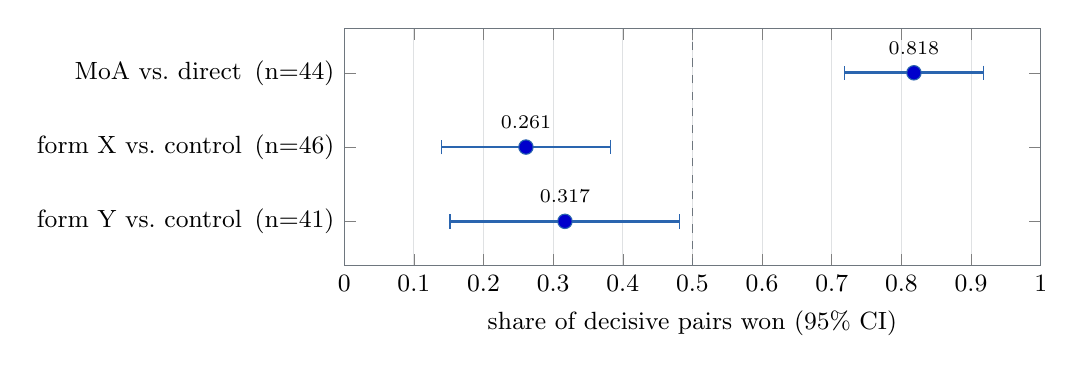
\begin{tikzpicture}
\begin{axis}[width=0.86\textwidth,height=4.6cm,xmin=0,xmax=1,
  ytick={1,2,3},yticklabels={form Y vs.\ control\, (n=41),
  form X vs.\ control\, (n=46), MoA vs.\ direct\, (n=44)},
  ymin=0.4,ymax=3.6,xlabel={share of decisive pairs won (95\% CI)},
  tick label style={font=\small},xlabel style={font=\small},
  axis line style={inkmut},xmajorgrids,grid style={inkmut!22}]
\addplot+[only marks,mark=*,mark size=2.6pt,color=accent,
  error bars/.cd,x dir=both,x explicit,error bar style={line width=1pt}]
  coordinates {
  (0.818,3) +- (0.100,0.101)
  (0.261,2) +- (0.121,0.127)
  (0.317,1) +- (0.165,0.163)};
\addplot[dashed,inkmut] coordinates {(0.5,0.4) (0.5,3.6)};
\node[font=\scriptsize,anchor=south] at (axis cs:0.818,3.12) {0.818};
\node[font=\scriptsize,anchor=south] at (axis cs:0.261,2.12) {0.261};
\node[font=\scriptsize,anchor=south] at (axis cs:0.317,1.12) {0.317};
\end{axis}
\end{tikzpicture}
\caption{The preference experiment (order-debiased; a pair is decisive
only when the same side wins both orderings; cluster-bootstrap CIs over
cases). The aggregated pipeline beats the matched-length direct
baseline decisively; both phrase-instructed arms lose to their own
control, in counterbalanced forms whose only difference from control is
the phrase. The dashed line is indifference.}
\label{fig:pref}
\end{figure}

\subsection{Design}

Three pairwise comparisons were run on the same 18 cases (126 pairs
each; both orderings; decisive only when the same side wins both;
primary judge \texttt{gpt-oss:20b}, which also wrote every output on
both sides of every pair, making self-preference symmetric by
construction). Comparison C1 pairs the phrase-swap control arm (the
two-layer MoA) against a generated direct arm: the same writer, same
cases, and same sampling, with the writer prompt minus only the
sentence referencing contributions. Comparisons C2 and C3 pair each
instructed arm against control. Because Section~\ref{sec:phrase}
established that those arms differ only in the phrase, any preference
gap is causally attributable to the phrase.

\subsection{Results}

\paragraph{The lift replicates at 20B scale.} The aggregated side wins
$0.818$ \ci{0.718}{0.919} of 44 decisive pairs. Arm mean lengths differ
by $1.4\%$ (7{,}757 versus 7{,}649 characters), and the share among
near-length-matched pairs is $0.815$, so the lift is not length
(Figure~\ref{fig:pref}). It also does not track domain-framework
density: the winner has more frameworks per kilocharacter in only
$0.409$ of decisive pairs. Its composition is unidentified by the
available feature set and is reported as such.

\paragraph{The phrase arms lose, in both forms.} The instructed arms'
shares against their own control are $0.261$ \ci{0.140}{0.388} (form
X) and $0.317$ \ci{0.152}{0.480} (form Y). Both confidence intervals
lie entirely below $0.5$, in the same direction, across counterbalanced
forms, and the penalty survives length matching. The registered
prediction was the opposite (that judges reward the compliance
register); the result is a falsification by reversal, and it is
stronger than the prediction: dictated epistemic marking costs
preference points.

\paragraph{Cross-family replication.} A second judge from a disjoint
model family (a 30B Qwen3 MoE), selected from three candidates blind to
direction (the pilot measured only parse and decisive rates, and the
selection script never computed which side won), re-judged all 378
pairs. The lift replicates: $0.788$ \ci{0.645}{0.917} ($n{=}33$
decisive). The form-Y penalty replicates: $0.217$ \ci{0.125}{0.333}
($n{=}23$). The form-X penalty agrees in point estimate ($0.276$ versus
$0.261$), but its interval spans $0.5$ at $n{=}29$ decisive and is
reported, per the registration, as not replicated at this power, a
category distinct from contradiction; no comparison lands on the
opposite side. The lift is therefore a two-family result, and the
phrase penalty holds in three of four judge-by-form cells.

\paragraph{The tension.} Chaining Sections~\ref{sec:phrase} and
\ref{sec:pref}, with both links causal: an epistemic instruction
installs only a surface form, and a preference judge penalizes that
form. A pipeline tuned toward judge preference, whether RLHF-style or
best-of-$n$ against a preference model, will therefore shed exactly the
epistemic marking that instruction paradigms install, while leaving the
underlying disposition (unchanged by the instruction in any case)
untouched. Preference optimization and epistemic disposition are not
merely unaligned; at this scale they are measurably opposed at the
surface where instructions act.

\section{Mechanisms the MoA Narrative Assumes}
\label{sec:mech}

\begin{figure}[t]
\centering
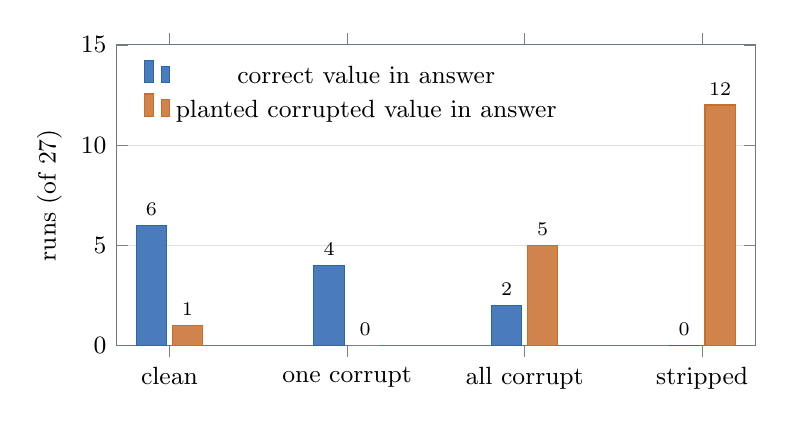
\begin{tikzpicture}
\begin{axis}[width=0.8\textwidth,height=5.4cm,ybar,bar width=11pt,
  ymin=0,ymax=15,ylabel={runs (of 27)},
  symbolic x coords={clean,one corrupt,all corrupt,stripped},xtick=data,
  axis line style={inkmut},tick label style={font=\small},
  ylabel style={font=\small},ymajorgrids,grid style={inkmut!22},
  legend style={font=\small,draw=none,at={(0.03,0.97)},anchor=north west},
  nodes near coords,nodes near coords style={font=\scriptsize,text=black}]
\addplot+[fill=accent!85,draw=accent] coordinates {
  (clean,6) (one corrupt,4) (all corrupt,2) (stripped,0)};
\addplot+[fill=corrupt!85,draw=corrupt] coordinates {
  (clean,1) (one corrupt,0) (all corrupt,5) (stripped,12)};
\legend{correct value in answer,planted corrupted value in answer}
\end{axis}
\end{tikzpicture}
\caption{The source-selector gradient (planted arithmetic errors; exact
match on known values). As clean sources are removed (one proposer
corrupted, all corrupted, working stripped), adoption of the planted
wrong value rises monotonically through $1$, $0$, $5$, and $12$ runs
while correct values vanish. The aggregator prefers uncorrupted sources
when they exist and has no independent hold on the content when they
do not.}
\label{fig:grad}
\end{figure}

\paragraph{The aggregator selects sources; it does not recompute.} With
arithmetic claims planted in proposer texts: when one proposer is
corrupted and a clean one remains, the corrupted value reaches the
answer $0/27$ times; when every proposer is corrupted, $5/27$; when the
working is also stripped, $12/27$. The monotone gradient across arms
($1$, $0$, $5$, $12$; Figure~\ref{fig:grad}) identifies a preference
for uncorrupted sources with no independent recomputation. MoA's own
evidence that the aggregator's output overlaps most with the best
proposals \cite{wang2024moa} is the same phenomenon viewed from the
benign side. The planted-error view adds its failure boundary and shows
that the claim of collaborativeness even from worse inputs fails at the
fact level: worse inputs made the writer factually worse.

\paragraph{Corroboration is ignored.} Claims advanced by $k\ge2$
independent proposers transport to the final answer no more often than
single-proposer claims ($0.487$ versus $0.524$; difference CI
\ci{-0.153}{+0.080}, excluding gains above $+0.08$). The one
reliability signal the architecture uniquely provides is unused.

\begin{figure}[t]
\centering
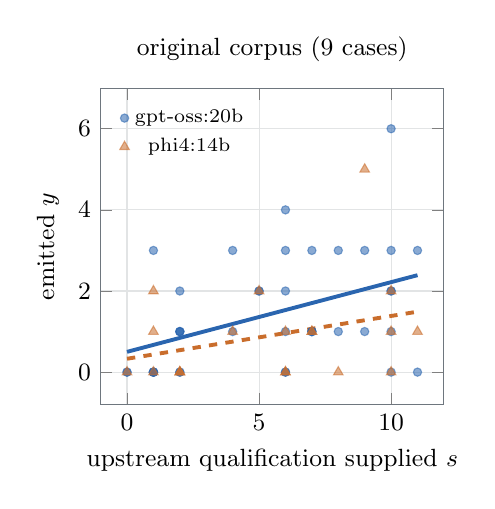
\begin{tikzpicture}
\begin{axis}[width=0.49\textwidth,height=5.6cm,
  xmin=-1,xmax=12,ymin=-0.8,ymax=7,
  xlabel={upstream qualification supplied $s$},ylabel={emitted $y$},
  title={\small original corpus (9 cases)},
  axis line style={inkmut},tick label style={font=\small},
  xlabel style={font=\small},ylabel style={font=\small},
  ymajorgrids,xmajorgrids,grid style={inkmut!20},legend style={font=\scriptsize,draw=none,at={(0.03,0.97)},anchor=north west,fill=none},]
\addplot[only marks,mark=*,mark size=1.5pt,color=accent,opacity=0.55]
  coordinates {(1.0,0.0) (1.0,0.0) (1.0,3.0) (1.0,0.0) (8.0,1.0) (8.0,3.0) (10.0,1.0) (10.0,0.0) (10.0,3.0) (10.0,2.0) (11.0,3.0) (11.0,0.0) (6.0,3.0) (6.0,1.0) (7.0,3.0) (7.0,1.0) (5.0,2.0) (5.0,2.0) (6.0,2.0) (6.0,0.0) (4.0,1.0) (4.0,3.0) (2.0,1.0) (2.0,2.0) (6.0,0.0) (6.0,4.0) (7.0,1.0) (7.0,1.0) (2.0,1.0) (2.0,1.0) (9.0,1.0) (9.0,3.0) (10.0,6.0) (10.0,2.0) (0.0,0.0) (0.0,0.0) (2.0,0.0) (2.0,0.0) (1.0,0.0) (1.0,0.0)};
\addplot[only marks,mark=triangle*,mark size=2pt,color=corrupt,opacity=0.55]
  coordinates {(1.0,1.0) (1.0,2.0) (8.0,0.0) (10.0,1.0) (10.0,2.0) (11.0,1.0) (6.0,0.0) (7.0,1.0) (5.0,2.0) (6.0,1.0) (4.0,1.0) (2.0,0.0) (6.0,0.0) (7.0,1.0) (2.0,0.0) (9.0,5.0) (10.0,0.0) (0.0,0.0) (2.0,0.0) (1.0,0.0)};
\addplot[accent,line width=1.4pt] coordinates {(0.0,0.50) (11.0,2.39)};
\addplot[corrupt,line width=1.4pt,dashed] coordinates {(0.0,0.33) (11.0,1.49)};
\legend{gpt-oss:20b,phi4:14b}
\end{axis}
\end{tikzpicture}\hfill
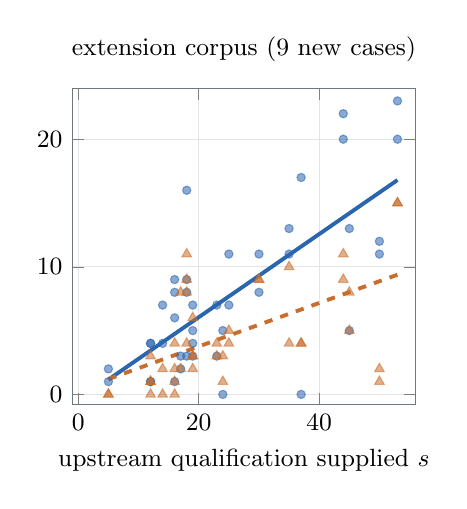
\begin{tikzpicture}
\begin{axis}[width=0.49\textwidth,height=5.6cm,
  xmin=-1,xmax=56,ymin=-0.8,ymax=24,
  xlabel={upstream qualification supplied $s$},
  title={\small extension corpus (9 new cases)},
  axis line style={inkmut},tick label style={font=\small},
  xlabel style={font=\small},ylabel style={font=\small},
  ymajorgrids,xmajorgrids,grid style={inkmut!20},]
\addplot[only marks,mark=*,mark size=1.5pt,color=accent,opacity=0.55]
  coordinates {(5,1) (5,2) (12,4) (12,4) (12,1) (12,1) (18,9) (18,8) (18,16) (18,3) (19,7) (19,4) (23,3) (23,7) (44,22) (44,20) (53,20) (53,23) (16,8) (16,9) (16,6) (16,1) (14,4) (14,7) (24,0) (24,5) (19,3) (19,5) (17,2) (17,3) (25,11) (25,7) (37,17) (37,0) (50,11) (50,12) (30,11) (30,8) (35,11) (35,13) (45,5) (45,13)};
\addplot[only marks,mark=triangle*,mark size=2pt,color=corrupt,opacity=0.55]
  coordinates {(5,0) (5,0) (12,3) (12,0) (12,1) (12,1) (18,11) (18,8) (18,9) (18,4) (19,3) (19,6) (23,4) (23,3) (44,11) (44,9) (53,15) (53,15) (16,0) (16,2) (16,1) (16,4) (14,0) (14,2) (24,1) (24,3) (19,2) (19,3) (17,8) (17,2) (25,5) (25,4) (37,4) (37,4) (50,2) (50,1) (30,9) (30,9) (35,4) (35,10) (45,5) (45,8)};
\addplot[accent,line width=1.4pt] coordinates {(5,1.16) (53,16.80)};
\addplot[corrupt,line width=1.4pt,dashed] coordinates {(5,1.20) (53,9.38)};

\end{axis}
\end{tikzpicture}
\caption{The transport coefficient $y = ws + c$, 144 runs over 18 cases
and two writers. Each point is one run: upstream epistemic
qualification supplied by the seats against qualification emitted by
the writer, both counted by the validated two-judge sentence protocol.
Lines are within-panel least-squares fits. The panels are separated
because the two corpora occupy different supply regimes (mean $s$ of
$5.4$ against $25.3$); pooling them produces a slope that is
essentially the line between the two clusters, so no pooled fit is
drawn. Within-panel slopes: \mbox{gpt-oss} $0.172$
\ci{+0.052}{+0.297} and $0.326$ \ci{+0.207}{+0.434}; phi4 $0.105$
\ci{-0.031}{+0.273} and $0.170$ \ci{+0.067}{+0.265}. Three of the four
exclude zero, and phi4's right-hand fit is an independent replication
on nine cases the original corpus never contained. The writer emits a
small fraction of what it is given, and the fraction is a property of
the writing step rather than of one model.}
\label{fig:transport}
\end{figure}

\paragraph{Transport is weak; invention is real.} On de-scaffolded arms
under the validated instrument, the writer transports only a small
fraction of the epistemic qualification it is given, and the relation
is linear over the observed range (Figure~\ref{fig:transport}).
Within-corpus slopes run from $0.105$ to $0.326$ across two writers and
two corpora, three of four excluding zero, with phi4's
extension-corpus fit of $0.170$ \ci{+0.067}{+0.266} replicating on nine
cases the original corpus never contained. The observed slope is an
attenuated lower bound: supply is judge-measured with inter-judge
$r = 0.528$, and correcting for that attenuation on the original corpus
moves $0.150$ to $0.217$. Pooling the two corpora is declined, because
their supply regimes differ by a factor of five and the pooled slope
reduces to the line between the two clusters. The writer also invents
qualification at a rate of $0.333$ \ci{0.138}{0.609} on inputs
confirmed to contain none, an independent estimate that falls inside
the intercept's interval.

\paragraph{Mixing is not automatically diverse.} Two medical fine-tunes
of the same base model do not share a domain signature: one shifts
in-domain framework density $+0.232$ \ci{+0.072}{+0.412} over the base,
the other $+0.109$ \ci{-0.056}{+0.300}, and a second lineage shows
$-0.041$ \ci{-0.099}{+0.025}. Signatures are per-model rather than
per-domain-training. A post-hoc descriptive check (not a registered
result) further found two same-domain seats no more distant from each
other than one seat is from itself across samples. Registered or not,
the published Self-MoA result \cite{li2025selfmoa} independently
reaches the same conclusion at benchmark scale.

\paragraph{Accuracy.} On a 60-item self-verifying battery, the
aggregated pipeline and the bare writer are statistically
indistinguishable at a $0.92$ to $0.97$ ceiling. Two registered
follow-up batteries then targeted the ceiling itself: 36 multi-step
computation items and 30 rule-interaction items with script-computed
answers, each under a baseline-only difficulty screen. The direct
writer reached ceiling again at $0.977$ and $0.983$. Under the
pre-registered two-strikes rule, the question is resolved as untestable
for lack of headroom on well-specified items at this scale: a council
cannot add accuracy where the single writer already delivers it.

\section{Routed Re-consultation}
\label{sec:reconsult}

Everything above bounds or removes. This section reports the one
intervention in the program that survived its own registered test, and
the structural reason its coverage is bounded.

\paragraph{Design.} The aggregator writes its tension list first (the
synthesis scaffold mandates one, and 391 of 396 archived runs contain
it), and an orchestrator, not the aggregator's disposition, parses that
list and dispatches a follow-up to the implicated proposer. Three arms
were run over six planted tensions whose deciding fact is withheld from
round one: no clarification; a length-matched clarification that is
responsive in style but contains no deciding fact; and the same
clarification containing it. The middle arm exists because
Section~\ref{sec:phrase} makes the alternative live: consultation could
shift behavior as ceremony rather than content.

\paragraph{Result.} On runs where the tension was named, the aggregator
adopted the fact-implied resolution in $7/7$ informed runs against
$0.333$ in control (cluster-bootstrap difference CI \ci{+0.200}{+1.000})
and $0.200$ under the contentless clarification (\ci{+0.545}{+0.947}).
The information does the work, not the ritual. The informed arm was
unanimous across both judges; resolving every judge disagreement in the
other arms adversarially against the prediction still leaves gaps of
$+0.40$ and $+0.53$; and emission is flat across arms.

This result is coherent with every failure above rather than an
exception to them. Instructions install phrases
(Section~\ref{sec:phrase}); corroboration is ignored
(Section~\ref{sec:mech}); the aggregator cannot verify
(Section~\ref{sec:mech}). Routed re-consultation is the only
intervention tested that operates through the one capability the
aggregator demonstrably has, preference among overlapping sources, by
manufacturing an uncorrupted source exactly at the contested quantity.

\paragraph{Why coverage is bounded: the trigger is scarce on planted
tensions.} On organic inquiries the picture is more favorable: in the
bundle comparison's 54 live pipelines, the orchestrator found a
role-named tension and dispatched on $0.85$ of runs, so planted-tension
rates are the floor rather than the forecast. A companion experiment
asked whether proposers can initiate the loop themselves, giving each a
roster and a structured deferral token, then putting the identical
sub-question to the proposer whose domain holds the deciding
consideration and to one whose domain does not. Routing, when it fires,
is accurate: the named domain is the correct one in $10/11$ cases,
$0.909$ \ci{0.623}{0.984} against a two-alternative chance rate of
$0.5$. But discrimination fails: flag rates are $0.306$ out-of-domain
against $0.083$ in-domain, a gap whose cluster-bootstrap CI
\ci{-0.056}{+0.528} spans zero, and the in-domain flags are a proposer
failing to recognize its own competence.

The experiments share one shape (Table~\ref{tab:trigger}).

\begin{table}[t]
\centering\small
\begin{tabular}{lcc}
\toprule
 & Mechanism, when triggered & Trigger rate \\
\midrule
aggregator uses a clarification & $7/7$ & $0.34$ names the tension \\
proposer routes a deferral & $0.909$ correct & $0.306$ recognizes the need \\
briefed proposer conveys, live & $21/21$ conveyed, $0.905$ adopted &
  $0.208$ to $0.583$ by batch \\
\bottomrule
\end{tabular}
\caption{Re-consultation is recognition-limited rather than
capability-limited: in each design the mechanism works when fired, and
the firing is rare.}
\label{tab:trigger}
\end{table}

\paragraph{Re-consultation is recognition-limited, not
capability-limited.} This is why the orchestrator-routed design is the
one recommended and the proposer-initiated design is not. The routed
design draws its trigger from a mandated artifact the aggregator
already produces, rather than from a model's assessment of its own
competence, the one faculty for which the program never found evidence.

\paragraph{The loop closes end-to-end with a live proposer.} The
results above used controlled clarification texts; two further
registered experiments replaced them with a real proposer. The first
buried the deciding fact in the proposer's own round-one contribution
and halted at its registered pilot gate: with the fact visible in the
pile, the tension was named in only $0.208$ of runs. This is recorded
as the halt, with the suppression mechanism left unproven. The second
restored the original round-one bytes and supplied the fact only as the
proposer's private working notes at reply time, knowledge held but
never written. The live proposer conveyed the fact in $21/21$
dispatched replies, and the aggregator adopted the fact-implied
resolution in $0.905$ of tension-named runs against the archived
control's $0.333$ ($+0.571$ \ci{+0.139}{+0.912}), within $-0.095$
\ci{-0.227}{0.000} of the scripted ceiling. Production, conveyance, and
use all work with no controlled inputs; what varies across batches is
only the trigger ($0.208$ to $0.583$ across the three experiments that
measured it, so no single rate should be quoted). One risk accompanied
the result: $4/21$ live replies embellished the correctly conveyed fact
with fabricated legal authority (invented case law, invented regulatory
rulings), and the aggregator adopted regardless. A content gate screens
absent content, not invented content. A registered follow-up
experiment bounded the rate at $0.100$ to $0.150$ reply-level,
concentrated on a single trigger topic and name-stable across
independent samples, with the gap never self-admitted ($0/20$ sampled
replies).

\paragraph{Scope.} Six items throughout, one writer family, and a
conditioned $n$ of seven in the original decisive experiment, where
unanimity was the only way to clear an interval. The live experiment's
comparators are the original experiment's archived arms under a
registered, never-pooled fresh-batch check. The judge agreement bar
was met on the analysis population ($0.703$) and not overall ($0.583$);
both are reported. These are existence results about a mechanism, not
effect sizes for deployment.

\section{Design Consequences, Engineered and Re-tested}
\label{sec:harness}

A falsification program carries a second obligation: if the findings
are real, the design rules they imply should survive prospective tests
of their own. The audit was distilled into a runtime architecture (an
evidence-bound harness, released with the ledger), and an experiment
was then registered against each load-bearing component. The principal
results follow. Each is a single-factor causal design, and two of the
verdicts in this arc contradicted the design's own rationale.

\paragraph{Engineered redundancy is causal.} The source-selector
finding (Section~\ref{sec:mech}) implies that protection is coverage,
and coverage is a design variable. A registered experiment assigned a
load-bearing quantity to a second proposer as one factor.
Corrupted-value adoption fell from $0.900$ (sole-sourced, corrupted;
the sharpest no-verification number in the program) to $0.450$
(\ci{+0.200}{+0.725}), and the clean value was adopted (from $0.000$ to
$0.500$, \ci{+0.175}{+0.825}). This is selection rather than dilution.
Protection is bimodal across items; two candidate mechanisms for the
boundary were then registered and rejected in turn (prior plausibility
at $0.544$; a stable, near-unanimous elicited ownership map whose
prospective prediction landed at exactly $0.500$ against a descriptive
$0.895$, the confirmation experiment performing precisely the
anti-calcification work it exists for). The boundary remains open, and
the planner's guarantee is stated as expected value only.

\begin{figure}[t]
\centering
\begin{minipage}{0.44\textwidth}
\centering
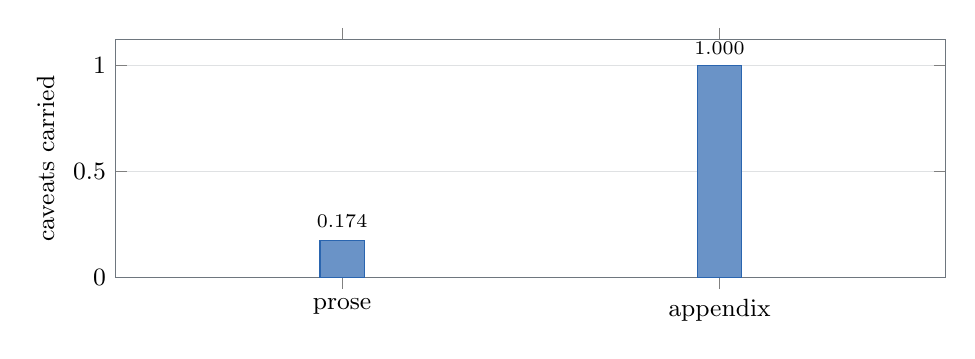
\begin{tikzpicture}
\begin{axis}[width=\textwidth,height=4.6cm,ybar,bar width=16pt,
  ymin=0,ymax=1.12,xtick={1,2},xticklabels={prose,appendix},
  ylabel={caveats carried},xmin=0.4,xmax=2.6,
  tick label style={font=\small},ylabel style={font=\small},
  axis line style={inkmut},ymajorgrids,grid style={inkmut!22}]
\addplot+[fill=accent!70,draw=accent] coordinates {(1,0.174) (2,1.000)};
\node[font=\scriptsize,anchor=south] at (axis cs:1,0.19) {0.174};
\node[font=\scriptsize,anchor=south] at (axis cs:2,1.005) {1.000};
\end{axis}
\end{tikzpicture}
\end{minipage}\hfill
\begin{minipage}{0.53\textwidth}
\centering
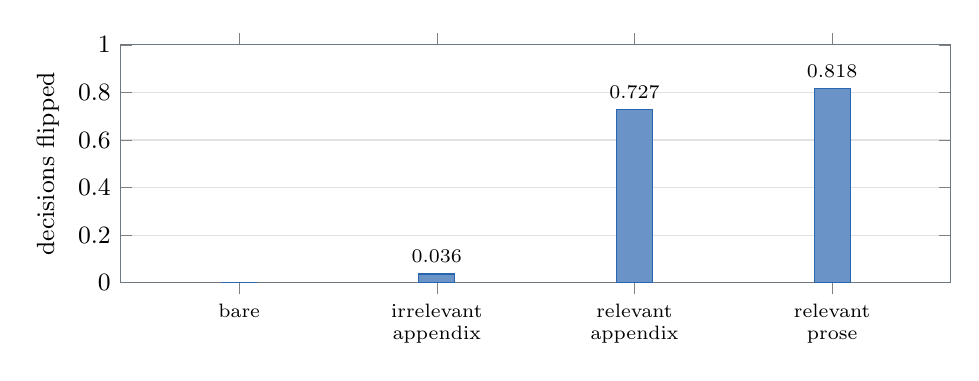
\begin{tikzpicture}
\begin{axis}[width=\textwidth,height=4.6cm,ybar,bar width=13pt,
  ymin=0,ymax=1.0,xtick={1,2,3,4},
  xticklabels={bare,{irrelevant\\appendix},{relevant\\appendix},
  {relevant\\prose}},xticklabel style={font=\scriptsize,align=center},
  ylabel={decisions flipped},xmin=0.4,xmax=4.6,
  tick label style={font=\small},ylabel style={font=\small},
  axis line style={inkmut},ymajorgrids,grid style={inkmut!22}]
\addplot+[fill=accent!70,draw=accent] coordinates
  {(1,0.000) (2,0.036) (3,0.727) (4,0.818)};
\node[font=\scriptsize,anchor=south] at (axis cs:2,0.045) {0.036};
\node[font=\scriptsize,anchor=south] at (axis cs:3,0.732) {0.727};
\node[font=\scriptsize,anchor=south] at (axis cs:4,0.823) {0.818};
\end{axis}
\end{tikzpicture}
\end{minipage}
\caption{The out-of-band channel, both halves. \emph{Left}: share of
both-judge caveat sentences reaching the final artifact through writer
prose against a mechanically assembled appendix (zero-generation
design; byte-identical prose in both arms). \emph{Right}: share of
registered two-token reader decisions flipped by a planted
decision-relevant caveat, by delivery arm (11 items, 440 reads; the
irrelevant-appendix arm carries a matched caveat that does not bear on
the decision). Uptake is content-specific ($+0.691$
\ci{+0.455}{+0.891} over the irrelevant control) and at parity with
in-prose placement ($+0.091$ \ci{-0.036}{+0.218}).}
\label{fig:freight}
\end{figure}

\paragraph{Out-of-band qualification carries, and is used.} The
transport and penalty results (Sections~\ref{sec:mech} and
\ref{sec:pref}) imply that epistemic qualification should never route
through the writer. The harness therefore carries proposer caveats in a
mechanically assembled appendix the writer never sees. Two registered
experiments tested the channel's halves (Figure~\ref{fig:freight}).
\emph{Carriage:} the appendix delivers $1.000$ of both-judge caveat
sentences against the $0.174$ that survives prose transport, with the
preference cost not evaluable at power ($0.510$ \ci{0.267}{0.754},
$65/116$ ties; no evidence of a penalty, and no license yet to claim
its absence). \emph{Uptake:} a decision-relevant caveat delivered
appendix-only flips a reader model's registered two-token decision in
$0.727$ of reads against $0.036$ for the identical appendix block
carrying an irrelevant caveat. The effect is content-specific rather
than caution-priming, with direction-balanced items (blocking and
enabling caveats) so that generic caution cannot masquerade as uptake,
and it is at parity with weaving the same sentence into prose. The
channel that preference pressure cannot see is not an exhibit: what it
carries changes decisions at no measured transport or preference cost.

\paragraph{An informative null demoted the isolation rule.} The harness
isolated proposers (task plus a one-line roster, never sibling outputs)
on the strength of a lane-bleed incident from an earlier pipeline
version. The registered one-factor test, with byte-fixed sibling
contributions made visible and production prompts otherwise unchanged,
found nothing: off-domain framework density moved $-0.009$
\ci{-0.048}{+0.028} against a pre-registered minimum detectable effect
of $+0.05$ to $+0.08$ computed from the archive, with in-domain density
unchanged. The isolation rule survives on cost grounds alone
(approximately $10$k input characters and $14\%$ longer outputs per
proposer, purchasing no measured change in lane discipline), and its
contamination rationale is withdrawn. This result is reported with the
same prominence as the positive results: the architecture documents
what its evidence failed to support, which is what distinguishes an
evidence-bound harness from a prompt stack.

\paragraph{The remaining components were closed out the same way.} The
seating gate's verdict at selection predicts pipeline defects (strict
rank separation over ten candidates, verdicts committed before any
pipeline run; pooled contrast $+0.632$ \ci{+0.549}{+0.722}), and gate
verdicts age: one model that passed an archived screen failed a fresh
re-gate and then defected in-pipeline exactly as the fresh verdict
predicted. The redundancy planner was measured link by link:
identification $0.633$, best on missing quantities ($0.813$);
assignment in $40/40$ plans; live conveyance at $0.85$ to $0.95$; and
end-to-end clean-source adoption of $+0.425$ \ci{+0.325}{+0.525}
against the planted $+0.500$. Live-reply fabrication was bounded
($0.10$ to $0.15$ reply-level, concentrated on a single trigger topic
and name-stable across samples, never self-admitted), licensing a
blocklist delivery filter that validated at $21$ true hits, $0$ false
positives, and $0$ misses over the reply archive. A content gate for
vacuous replies failed two registered attempts on complementary halves
and is recorded as not deployable. Finally, the assembled bundle was
compared head-to-head against the plain pipeline on the deployment
artifact: no evaluable preference difference (primary-judge share
$0.562$ \ci{0.375}{0.765}; large effects excluded both ways), with the
appendix's within-pair attribution mildly positive. The harness ships
its machinery at no detectable preference cost.

\section{Discussion}
\label{sec:discussion}

\paragraph{What the lift is, and is not.} The audit does not overturn
MoA's headline: aggregation genuinely wins preference at this scale,
under a debiased protocol, against a matched-length direct baseline.
What the audit removes is the assumed mechanism story. The lift is not
built from the epistemic behaviors the aggregate prompt requests (those
requests install phrases, and the judge penalizes them), not from
length, and not from domain-framework density; and the aggregator
beneath it selects rather than verifies. The residual, plausibly
organization, coverage, or specificity harvested from proposers, is the
right target for the next instrument, and it is not named here without
one. What the audit supplies constructively is
Section~\ref{sec:reconsult}: the gain available from an aggregation
pipeline lies not in instructing the aggregator to be careful, but in
routing a specific question back to a specific proposer at the moment a
specific claim is contested.

\paragraph{Implication for preference-trained pipelines.} The measured
tension predicts that preference optimization silently strips epistemic
marking. This is consistent with, and sharpens, verbosity- and
sycophancy-style results \cite{singhal2023length,sharma2023sycophancy}:
the pressure is not merely toward longer or more agreeable text but
away from the specific surface forms by which pipelines currently
signal uncertainty. Systems that must retain calibrated marking under
preference pressure will need it carried somewhere preference cannot
see, such as structured fields or tool outputs, rather than in-band
prose. This is no longer offered as advice alone: the out-of-band
channel is tested (Section~\ref{sec:harness}), carries everything prose
loses, changes downstream decisions, and shows no detected preference
cost.

\paragraph{Implication for evaluation.} At auditable scale, five sixths
of a raw preference verdict is reading order. Single-ordering LLM-judge
evaluations at this scale are measuring position; debiased protocols
are usable but must budget for a decisive rate of approximately
$0.35$.

\section{Limitations}
\label{sec:limits}

The primary preference judge is also the writer (symmetric within
pairs, but family-specific); the cross-family replication discharges
this for the lift and for the form-Y penalty, while the form-X penalty
rests on one family's interval plus a point-estimate agreement at lower
power. One aggregator family and 7 to 20B scale are used throughout;
the tension should be retested with larger judges. The case battery is
advisory-domain and English-only. The phrase-swap experiment's null
licenses only effects of at least $0.22$; the preference experiments'
decisive counts (44 and 33) give minimum detectable shares of
approximately $0.67$ to $0.70$, which the observed lifts clear but
subtler ones would not. Several early program values remain provisional
pending re-measurement and are not used here. The engineered-consequence
experiments (Sections~\ref{sec:reconsult} and \ref{sec:harness}) carry
their own bounds: cluster ceilings of 6 to 18 items; the uptake verdict
rests on 11 of 18 authored items after a registered floor gate; the
live-loop experiment compares against archived arms under a fresh-batch
check rather than concurrent regeneration; the redundancy boundary is
bimodal with its mechanism open after two registered attempts; the
isolation null covers sibling outputs, not cross-domain instruction
framing; and the live-reply fabrication rate is bounded only for
adversarial case citations. Trigger rates vary by batch ($0.208$ to
$0.583$) and are never optimization targets under the program's
Goodhart charter. Claims are stated with their judge-family scope and
should not be generalized past it.

\section{Conclusion}
\label{sec:conclusion}

This audit establishes three linked results about LLM aggregation
pipelines at auditable scale. An epistemic instruction to the
aggregator installs only its named phrase; order-debiased preference
judges penalize that phrase while rewarding aggregation itself; and the
preference instrument is dominated by reading order as a property of
the pairwise format. The mechanisms the MoA narrative assumes are
largely absent: the aggregator selects rather than verifies, ignores
corroboration, and transports a small fraction of the qualification it
receives. One intervention, orchestrator-routed re-consultation,
survived its registered test and closed end-to-end with a live
proposer. The design consequences of these findings were engineered
into an evidence-bound harness and prospectively re-tested, with the
demotions reported beside the confirmations. The measurement kit,
dictation registry, and complete pre-registration ledger are released
to support replication.

\section*{Reproducibility Statement}

The measurement kit (\texttt{gst}: record contracts, pure-stdlib
statistics, instruments, registry, and gates), the frozen dictation
registry and form-freeze files, all pre-registrations with their
falsification conditions and attainability computations, every
deviation and verdict, and the three program audits are in the project
repository. Each experiment's registration is committed before its
first run, so temporal ordering is verifiable from version history.

\begin{thebibliography}{9}
\bibitem{wang2024moa} J.~Wang, J.~Wang, B.~Athiwaratkun, C.~Zhang,
J.~Zou. Mixture-of-Agents enhances large language model capabilities.
\emph{arXiv:2406.04692}, 2024.
\bibitem{li2025selfmoa} W.~Li et al. Rethinking Mixture-of-Agents: is
mixing different large language models beneficial?
\emph{arXiv:2502.00674}, 2025.
\bibitem{zheng2023judging} L.~Zheng et al. Judging LLM-as-a-judge with
MT-Bench and Chatbot Arena. \emph{NeurIPS Datasets and Benchmarks},
2023.
\bibitem{singhal2023length} P.~Singhal et al. A long way to go:
investigating length correlations in RLHF. \emph{arXiv:2310.03716},
2023.
\bibitem{sharma2023sycophancy} M.~Sharma et al. Towards understanding
sycophancy in language models. \emph{arXiv:2310.13548}, 2023.
\bibitem{wang2024rebuttal} Q.~Wang et al. Rethinking the bounds of LLM
reasoning: are multi-agent discussions the key? \emph{arXiv:2402.18272},
2024.
\end{thebibliography}

\end{document}
